% In this section, we review and analyze related works. We begin with a review of graph convolutional models and then transition to graph attention models. Lastly, we discuss other works on graphs. 

\begin{figure*}[tb!] 
\centering
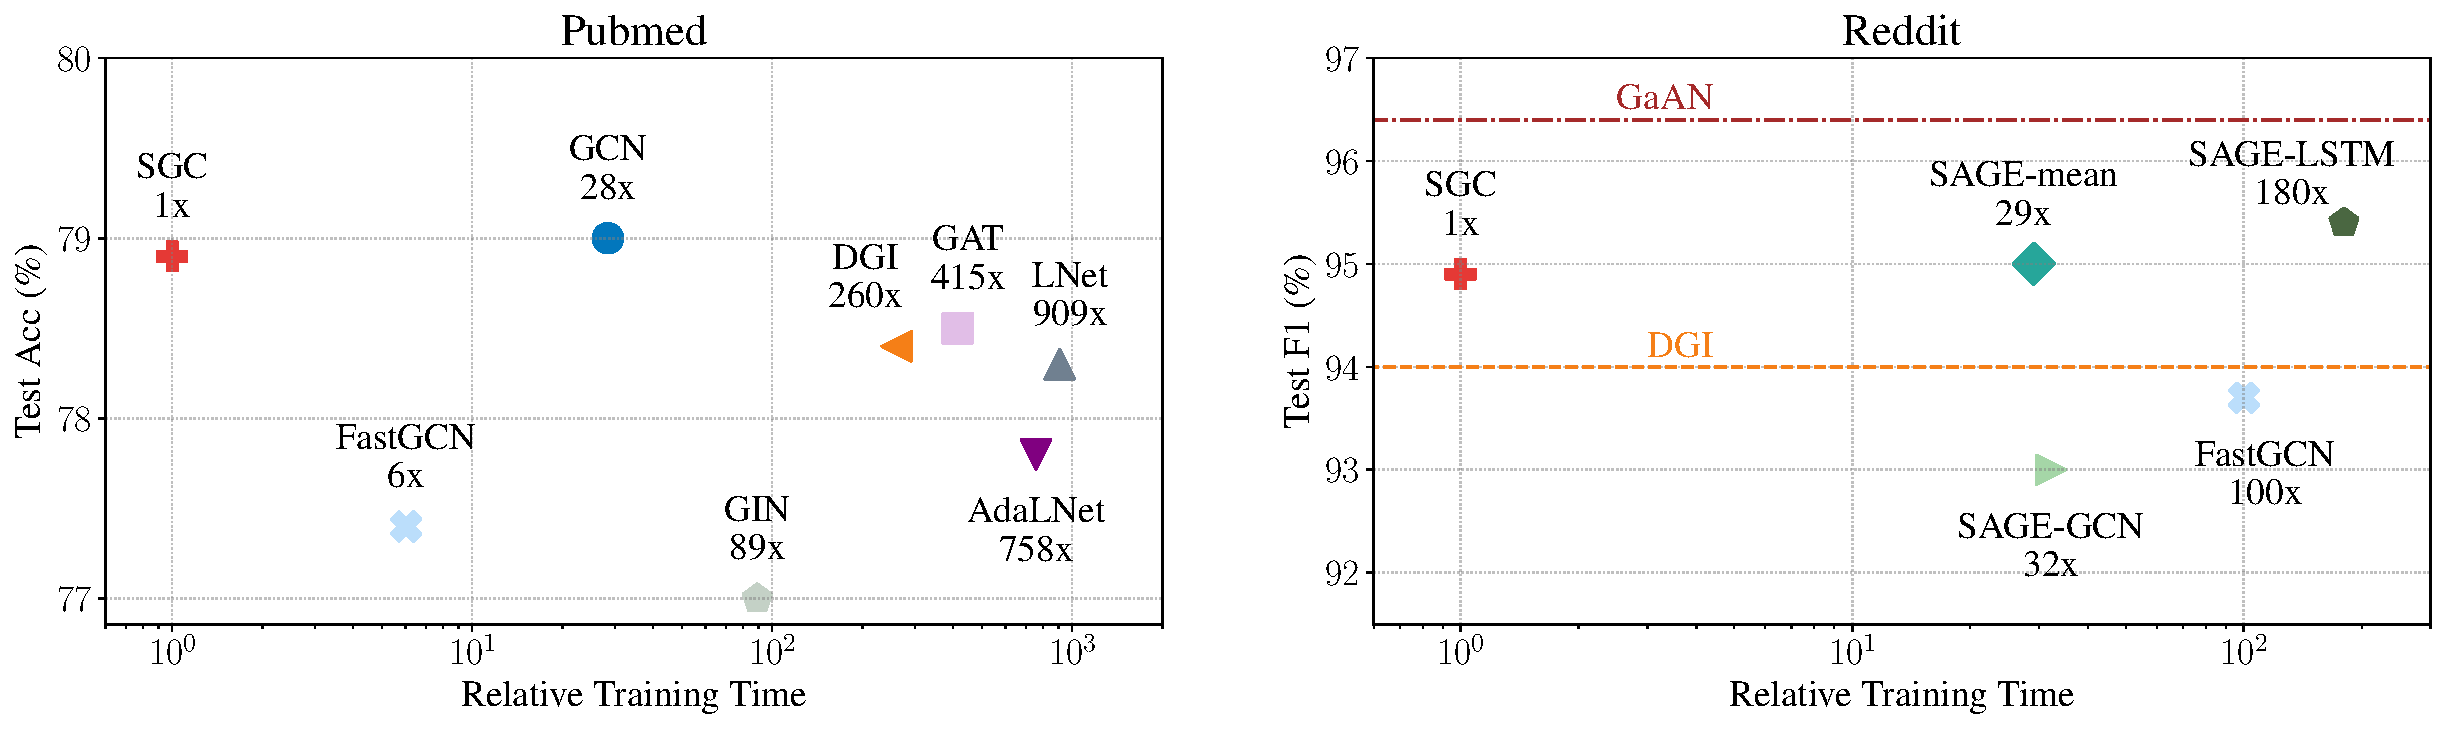
\includegraphics[width=0.8\textwidth]{acc_run_time_v2.pdf}
\caption{Performance over training time on Pubmed and Reddit. \method{} is the fastest while achieving competitive performance. 
We are not able to benchmark the training time of GaAN and DGI on Reddit because the implementations are not released. 
}
\label{fig:run_time}
\end{figure*}
%
\subsection{Graph Neural Networks}
\citet{Bruna13} first propose a spectral graph-based extension of convolutional networks to graphs. 
In a follow-up work, ChebyNets \cite{Defferrard16} define graph convolutions using Chebyshev polynomials to remove the computationally expensive Laplacian eigendecomposition. GCNs \cite{gcn} further simplify graph convolutions by stacking layers of first-order Chebyshev polynomial filters with a redefined propagation matrix $\mathbf{S}$. 
\citet{FastGCN} propose an efficient variant of GCN based on importance sampling, and \citet{Hamilton17} propose a framework based on sampling and aggregation. 
\citet{dcnn}, \citet{n-gcn}, and \citet{liao2018lanczosnet} exploit multi-scale information by raising $\mathbf{S}$ to higher order.
% \citet{xu2018how} introduce Graph Isomorphism Networks which is claimed to be the most expressive variant of GNNs.
\citet{xu2018how} study the expressiveness of graph neural networks in terms of their ability to distinguish any two graphs and introduce Graph Isomorphism Network, which is proved to be as powerful as the Weisfeiler-Lehman test for graph isomorphism. 
\citet{Klicpera19} separate the non-linear transformation from propagation by using a neural network followed by a personalized random walk.
There are many other graph neural models~\cite{Monet, EP17, Li18}; we refer to \citet{gnn_review, battaglia2018relational, wu2019comprehensive} for a more comprehensive review. 

% GLN
% \citet{agnn} discover that a linear version of GCN can perform competitively and develop a attention-based GCN model.
% \citet{cai2018simple} propose an effective linear baseline for graph classification using node degree statistics.
% \citet{Buchnik18} show that self-training can improve the base linear graph model.
% \citet{Li2019LabelES} propose a generalized version of label propagation and provide a similar spectral analysis on the renormalization trick.

Previous publications have pointed out that simpler, sometimes linear models can be effective for node/graph classification tasks. \citet{agnn} empirically show that a linear version of GCN can perform competitively and propose an attention-based GCN variant. \citet{cai2018simple} propose an effective linear baseline for graph classification using node degree statistics. \citet{Buchnik18} show that models which use linear feature/label propagation steps can benefit from self-training strategies. 
\citet{Li2019LabelES} propose a generalized version of label propagation and provide a similar spectral analysis of the renormalization trick.
% Unlike these previous works, we ...


% Recently, \citet{agnn} proposed an attention-based GCN model for citation networks. The authors point out that a linear version of GCN could perform similarly to GCNs on these classification tasks, which matches our findings. \citet{cai2018simple} propose an effective linear baseline for non-attribute graph classification using simple node degree statistics.

% \subsection{Graph Attention Models}
Graph Attentional Models learn to assign different edge weights at each layer based on node features and have achieved state-of-the-art results on several graph learning tasks \citep{gat, agnn, zhang2018gaan, ADGPM}.
However, the attention mechanism usually adds significant overhead to computation and memory usage. 
We refer the readers to \citet{attention-survey} for further comparison.

\subsection{Other Works on Graphs} 
Graph methodologies can roughly be categorized into two approaches: graph embedding methods and graph laplacian regularization methods. 
Graph embedding methods \citep{Weston2008, Perozzi14, Yang16, infomax} represent nodes as high-dimensional feature vectors. 
Among them, DeepWalk~\citep{Perozzi14} and Deep Graph Infomax (DGI)~\citep{infomax} use unsupervised strategies to learn graph embeddings.
DeepWalk relies on truncated random walk and uses a skip-gram model to generate embeddings, whereas DGI trains a graph convolutional encoder through maximizing mutual information. 
Graph Laplacian regularization \citep{Zhu03, Zhou04,Belkin04b,Belkin2006} introduce a regularization term based on graph structure which forces nodes to have similar labels to their neighbors.
Label Propagation~\citep{Zhu03} makes predictions by spreading label information from labeled nodes to their neighbors until convergence. 